\vspace{-12pt}
\section{Introduction}\label{sect:intro}
\vspace{-4pt}

Our investigation begins with a thought experiment. Imagine a deep neural network with capacity 1000 times greater than today's most powerful architectures: for example, a language model trained on all digitally available texts or a generative model for all images ever uploaded to the Internet. How can we train such a model?

\vspace{-1.5pt}

Viewed from a historical perspective, the 1000-fold increase in capacity is not unrealistic. Over the past decade, the deep learning community has made remarkable progress by training large models on abundant data, and the scale of those models keeps growing. Since the advent of the ImageNet challenge \cite{imagenet_cvpr09} with 1.3M labeled images, the typical size of convolutional neural networks increased from a few megabytes to hundreds of megabytes \cite{alexnet, resnet, huang2019gpipe}. Recent studies report even larger models for datasets with hundreds of millions of images \cite{kolesnikovlarge, jft300data}.

\vspace{-1.5pt}

Another trend from natural language processing is to train large Transformer-like language models~\cite{bert, roberta, kaplan2020scaling}. The data for this task is nearly unlimited, allowing researchers to train models with tens or even hundreds of gigabytes of parameters~\cite{brown2020language,shoeybi2019megatron,zellers2019defending,tnlg}. While we may not need the 1000-fold increase at the moment, planning for it will prepare us for the next big leap in model capacity.

\vspace{-1.5pt}

To be specific, let us focus on training large Transformer networks for the language modeling task. At the time of writing, the largest conventional model for that task is GPT-3 with 175 billion parameters. Scaling it up 1000 times gives us 175 trillion; depending on whether you use single or half-precision, this requires 300--600 terabytes of memory just to store the model. No modern mass-produced hardware accelerator is up to such task. Even high-end servers with 16x V100 accelerators can store only 0.15\% of that model in combined GPU memory, let alone train it.

The dominant way of growing neural network size has so far been to scale up: deploy more powerful computational accelerators in specialized tightly interconnected clusters. However, this approach will only work up to a point. Models such as T-NLG~\cite{tnlg} and Megatron-LM~\cite{shoeybi2019megatron} were already trained on DGX-SuperPOD --- a supercomputer with hundreds of Tesla V100 GPUs spread over tens of servers. As for GPT-3~\cite{brown2020language}, a single \textit{training run} was estimated to cost 4.6 -- 12 million dollars~\cite{gpt3costlambda,gpt3cost}. 

Even today, the need for costly hardware weighs heavily on the research community. Most researchers cannot contribute to the development of large neural networks because conducting the necessary experiments would be too expensive for them. If we continue to increase the model size by scaling up, eventually the only labs that can conduct competitive research will be those with massive budgets.

However, there is another solution: to scale out. Instead of using a supercomputer, researchers could crowdsource the computation from volunteers with regular PCs. %
This paradigm is known as volunteer computing and was successfully applied to solve problems in biology \cite{larson_crowd}, high energy physics \cite{adam2015atlas} and other subject areas. While a single volunteer PC may be slow and unreliable, the combined floating-point performance of such projects is on par with largest supercomputers \cite{gross_folding}.

The main challenge of volunteer computing is how to utilize this performance. Unlike server pods, consumer-grade PCs communicate over the Internet, which is significantly slower, especially in terms of latency. They are also more prone to failures as they lack many reliability features of their server-grade counterparts. Therefore, volunteer computing was traditionally used for tasks that have high computation to communication ratio and can recover from individual node failures.

Unfortunately, existing paradigms of distributed training require nodes to continuously transfer large amounts of intermediate data \cite{Dettmers20158BitAF,Sun2019OptimizingNP}, making them unsuitable for volunteer computing. In this work, we take a different approach. Instead of adopting the existing distributed training strategies, we identify the advantages of volunteer computing and design a new strategy that capitalizes on them.

We summarize the contributions of our paper as follows:

\vspace{-6px}
\begin{minipage}{0.55\textwidth}

\begin{itemize}[leftmargin=*]
    \item We propose Decentralized Mixture of Experts (DMoE) --- a layer designed for training with vast amounts of unreliable consumer-grade hardware;%
    \vspace{1px}\item We describe a framework for training large neural networks composed of DMoE layers;%
    \vspace{1px}\item We confirm the efficiency and reliability of this approach using formal guarantees and experiments;
    \vspace{1px}\item The PyTorch source code that can be used to reproduce our results is available online\footnotemark.
\end{itemize}
\end{minipage}
\hspace{5px}
\begin{minipage}{0.45\textwidth}
\vspace{-6px}
    \centering
    \raisebox{\dimexpr \topskip-\height}{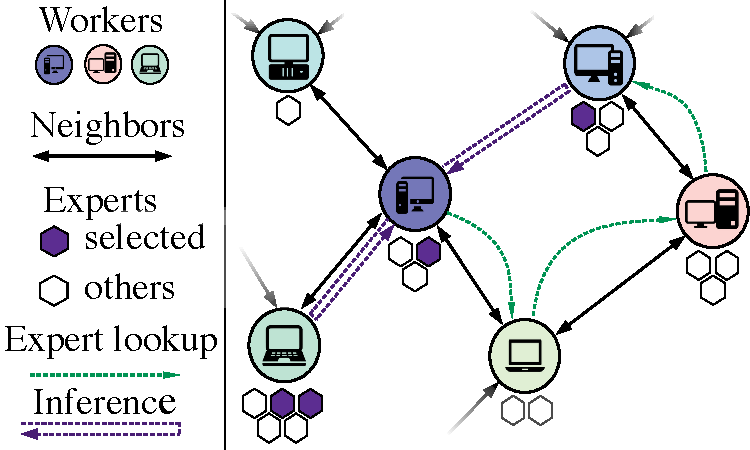
\includegraphics[width=180px]{resources/teasseract3.pdf}}
    \captionof{figure}{High-level scheme of Decentralized Mixture of Experts. See Section \ref{sect:method} for details.}
    \label{fig:teaser}
\end{minipage}
\footnotetext{\url{https://github.com/mryab/learning-at-home}}